\documentclass[12pt]{article}
\usepackage[]{graphicx}
\usepackage[]{color}
\usepackage{alltt}

\newcommand{\mytitle}{Bayesian (Generalized) Linear Models}
\newcommand{\myname}{Lona Koers}
\newcommand{\mysupervisor}{Dr. Ludwig Bothmann}

\usepackage[a4paper, width = 160mm, top = 35mm, bottom = 30mm,
bindingoffset = 0mm]{geometry}
\usepackage[utf8]{inputenc}
\usepackage{ragged2e}
\usepackage{xcolor}
\usepackage[round, comma]{natbib}
% \usepackage[authoryear,comma]{natbib}
\usepackage{har2nat}
\usepackage{fancyhdr}
\usepackage{hyperref}
\newcommand{\changefont}{%
    \fontsize{8}{11}\selectfont
}
\usepackage{amsmath}
\usepackage[nameinlink]{cleveref}
\usepackage{booktabs}
\usepackage[font=scriptsize,labelfont=bf]{caption}
\hypersetup{
  colorlinks = true,
  linkcolor = black,
  urlcolor = black,
  citecolor = black}
\pagestyle{fancy}
\fancyhead{}
\fancyhead[R]{\changefont{\mytitle}}
\fancyfoot{}
\fancyfoot[R]{\thepage}
\setlength{\headheight}{14.5pt}
\setlength{\parindent}{0pt}
\interfootnotelinepenalty = 10000

\usepackage{bm}
\usepackage{dsfont}
\usepackage{amssymb}
\usepackage{accents}
\usepackage[T2A,T1]{fontenc}


% bold letters (vectors)
\newcommand{\bnull}{\bm{0}}
\newcommand{\ba}{\bm{a}}
\newcommand{\bb}{\bm{b}}
\newcommand{\bc}{\bm{c}}
\newcommand{\bd}{\bm{d}}
\newcommand{\be}{\bm{e}}
% \newcommand{\bf}{\bm{f}}
\newcommand{\bg}{\bm{g}}
\newcommand{\bh}{\bm{h}}
\newcommand{\bi}{\bm{i}}
\newcommand{\bj}{\bm{j}}
\newcommand{\bk}{\bm{k}}
\newcommand{\bl}{\bm{l}}
% \newcommand{\bm}{\bm{m}}
\newcommand{\bn}{\bm{n}}
\newcommand{\bo}{\bm{o}}
\newcommand{\bp}{\bm{p}}
\newcommand{\bq}{\bm{q}}
\newcommand{\br}{\bm{r}}
\newcommand{\bs}{\bm{s}}
\newcommand{\bt}{\bm{t}}
\newcommand{\bu}{\bm{u}}
\newcommand{\bv}{\bm{v}}
\newcommand{\bw}{\bm{w}}
\newcommand{\bx}{\bm{x}}
\newcommand{\by}{\bm{y}}
\newcommand{\bz}{\bm{z}}

% bold letters (matrices)
\newcommand{\bA}{\bm{A}}
\newcommand{\bB}{\bm{B}}
\newcommand{\bC}{\bm{C}}
\newcommand{\bD}{\bm{D}}
\newcommand{\bE}{\bm{E}}
% \newcommand{\bf}{\bm{f}}
\newcommand{\bG}{\bm{G}}
\newcommand{\bH}{\bm{H}}
\newcommand{\bI}{\bm{I}}
\newcommand{\bJ}{\bm{J}}
\newcommand{\bK}{\bm{K}}
\newcommand{\bL}{\bm{L}}
\newcommand{\bM}{\bm{M}}
\newcommand{\bN}{\bm{N}}
\newcommand{\bO}{\bm{O}}
\newcommand{\bP}{\bm{P}}
\newcommand{\bQ}{\bm{Q}}
\newcommand{\bR}{\bm{R}}
\newcommand{\bS}{\bm{S}}
\newcommand{\bT}{\bm{T}}
\newcommand{\bU}{\bm{U}}
\newcommand{\bV}{\bm{V}}
\newcommand{\bW}{\bm{W}}
\newcommand{\bX}{\bm{X}}
\newcommand{\bY}{\bm{Y}}
\newcommand{\hbY}{\hat{\bm{Y}}}
\newcommand{\bZ}{\bm{Z}}


% calligraphic letters
\newcommand{\Acal}{\mathcal{A}}
\newcommand{\Bcal}{\mathcal{B}}
\newcommand{\Ccal}{\mathcal{C}}
\newcommand{\Dcal}{\mathcal{D}}
\newcommand{\Ecal}{\mathcal{E}}
\newcommand{\Fcal}{\mathcal{F}}
\newcommand{\Gcal}{\mathcal{G}}
\newcommand{\Hcal}{\mathcal{H}}
\newcommand{\Ical}{\mathcal{I}}
\newcommand{\Jcal}{\mathcal{J}}
\newcommand{\Kcal}{\mathcal{K}}
\newcommand{\Lcal}{\mathcal{L}}
\newcommand{\Mcal}{\mathcal{M}}
\newcommand{\Ncal}{\mathcal{N}}
\newcommand{\Ocal}{\mathcal{O}}
\newcommand{\Pcal}{\mathcal{P}}
\newcommand{\Qcal}{\mathcal{Q}}
\newcommand{\Rcal}{\mathcal{R}}
\newcommand{\Scal}{\mathcal{S}}
\newcommand{\Tcal}{\mathcal{T}}
\newcommand{\Ucal}{\mathcal{U}}
\newcommand{\Vcal}{\mathcal{V}}
\newcommand{\Wcal}{\mathcal{W}}
\newcommand{\Xcal}{\mathcal{X}}
\newcommand{\Ycal}{\mathcal{Y}}
\newcommand{\Zcal}{\mathcal{Z}}

% greek letters
\newcommand{\eps}{\varepsilon}
\newcommand{\sd}{\sigma}
\newcommand{\ssd}{\sigma^2}
\newcommand{\Sd}{\Sigma}
\newcommand{\Sdi}{\Sigma^{-1}}

\newcommand{\gb}[1]{\beta_#1}
\newcommand{\hbe}[1]{\hat{\beta}_#1}
\newcommand{\beps}{\bm{\varepsilon}}
\newcommand{\hbeps}{\hat{\bm{\varepsilon}}}

\newcommand{\balpha}{\bm{\alpha}}
\newcommand{\bbeta}{\bm{\beta}}
\newcommand{\hbbeta}{\hat{\bm{\beta}}}
\newcommand{\hssd}{\hat{\sigma^2}}
\newcommand{\bchi}{\bm{\chi}}
\newcommand{\bdelta}{\bm{\delta}}
\newcommand{\bepsilon}{\bm{\epsilon}}
\newcommand{\bphi}{\bm{\phi}}
\newcommand{\bgamma}{\bm{\gamma}}
\newcommand{\betah}{\bm{\etah}}
\newcommand{\bpi}{\bm{\pi}}


% prior and posterior parameters
\DeclareSymbolFont{cyrhelper}{T2A}{\familydefault}{m}{n}
\DeclareMathAccent{\post}{\mathord}{cyrhelper}{18}


\newcommand{\btheta}{\bm{\theta}}
\newcommand{\hbtheta}{\hat{\bm{\theta}}}

\newcommand{\thetapri}{\breve{\bm{\theta}}}
\newcommand{\thetapo}{\post{\bm{\theta}}}
\newcommand{\mupri}{\breve{\bm{\mu}}}
\newcommand{\mupo}{\post{\bm{\mu}}}
\newcommand{\Sdpri}{\breve{\Sigma}}
\newcommand{\Sdpo}{\post{\Sigma}}
\newcommand{\Sdipri}{\breve{\Sigma}^{-1}}
\newcommand{\Sdipo}{\post{\Sigma}^{-1}}

\newcommand{\apri}{\breve{a}}
\newcommand{\apo}{\post{a}}
\newcommand{\bpri}{\breve{b}}
\newcommand{\bpo}{\post{b}}

\newcommand{\btaus}{\bm{\tau}^2}
\newcommand{\taus}{\tau^2}


% other
\newcommand{\ty}{\tilde{\bm{y}}}
\newcommand{\tX}{\tilde{\bm{X}}}


\renewcommand{\bar}{\overline}


% statistics
\providecommand{\Pr}{}
\renewcommand{\Pr}{\mathbb{P}}
\newcommand{\Ex}{\mathbb{E}}
\newcommand{\var}{{\mathds{V}\mathrm{ar}}}
\newcommand{\cov}{{\mathds{C}\mathrm{ov}}}
\newcommand{\corr}{{\mathrm{Corr}}}
\newcommand{\ov}{\overline}
\newcommand{\wh}[1]{\widehat{#1}}
\newcommand{\wt}[1]{\widetilde{#1}}
\newcommand{\Cov}{\text{Cov}}
\newcommand{\IG}{\text{IG}}

\newcommand{\sumin}{\sum_{i = 1}^n}
\newcommand{\sumjn}{\sum_{j = 1}^n}
% ------------------------------------------------------------------------------
% MAIN -------------------------------------------------------------------------
% ------------------------------------------------------------------------------
\IfFileExists{upquote.sty}{\usepackage{upquote}}{}
\begin{document}

% FRONT PAGE -------------------------------------------------------------------

\begin{titlepage}
\begin{center}

\LARGE
Probabilistic Machine Learning

\vspace{0.5cm}

\rule{\textwidth}{1.5pt}
\LARGE
\textbf{\mytitle}
\rule{\textwidth}{1.5pt}

\vspace{0.5cm}

\large
Department of Statistics \\
Ludwig-Maximilians-Universität München

\vfill

\Large
\textbf{\myname}

\vfill

\large
Munich, 04. July 2025

\vfill


\includegraphics[width = 0.4\textwidth]{sigillum.png}

\vfill

\normalsize
Submitted as a seminar paper for the seminar on Probabilistic Machine Learning.
\\

Supervised by \mysupervisor

\end{center}
\end{titlepage}

% CONTENTS ---------------------------------------------------------------------

\pagenumbering{Roman}
\newpage

\begin{abstract}

  Bayesian generalized linear models (GLMs) offer a framework for incorporating uncertainty and prior knowledge into regression models.
  By placing prior distributions over parameters, they enable posterior-based uncertainty quantification and regularization.
  
  Especially in high-dimensional or low-information settings, regularization priors stabilize inference and improve generalization.
  However, the posterior distribution in Bayesian GLMs is often analytically intractable, which makes approximate inference methods necessary.

  This paper introduces the Bayesian view on linear and logistic regression while highlighting the role of regularization priors and comparing Laplace approximation and Markov chain Monte Carlo for posterior inference.
  Using synthetic data, we evaluate predictive performance and variable selection accuracy in low-information scenarios under different priors and compare different methods for posterior inference.
\end{abstract}

\newpage

\tableofcontents

\newpage

% CHAPTERS ---------------------------------------------------------------------

\pagenumbering{arabic}

\section{Introduction}
\label{sec:intro}
Generalized linear models (GLMs) are a fundamental tool in statistics and machine learning and are widely applied across various domains.
Their appeal lies in their simplicity, interpretability, and extensibility \citep{nelder_generalized_1972}.
However, GLMs also come with limitations:
They rely on maximum likelihood estimation (MLE), offer no mechanism for incorporating prior information or stabilizing inference \citep{gelman_weakly_2008}, and most importantly, only produce point estimates and thus cannot capture the full range of uncertainty in predictions and parameter estimates \citep{tyralis_review_2024}.\\

Bayesian GLMs take on a different viewpoint on GLMs to addresses these shortcomings.
They offer a natural way to quantify uncertainty with posterior distributions, which is especially useful in data-scarce scenarios.
For instance, \citet{sondhi_bayesian_2021} demonstrate this in precision oncology, where Bayesian inference compensates for small sample sizes and stabilizes confidence estimation in effect sizes.
Recent work has also shown that Bayesian regularization techniques can perform on par with or even outperform classic regularization, while also offering greater flexibility and interpretability \citep[see e.g.][]{van_erp_shrinkage_2019,celeux_regularization_2012}.
Additionally, a Bayesian framework allows for the incorporation of domain knowledge through informative priors.
For example, \citet{chien_informative_2023} outline a framework for constructing priors directly from expert knowledge or prior experiments.\\

This paper explores Bayesian GLMs as an alternative to classical approaches.
In \Cref{sec:bayesian_lm}, we introduce Bayesian linear regression as a familiar starting point within the Bayesian framework.
\Cref{sec:bayesian_logit} extends this foundation to generalized models, focusing on logistic regression as the most-used GLM.
\Cref{sec:simulation} illustrates the application of regularization and approximate inference methods in Bayesian GLMs using synthetic data experiments.\\




\newpage


\section{Bayesian Linear Model}
\label{sec:bayesian_lm}

The (frequentist) Linear Regression Model is probably the most well-known and most used statistical model. The frequentist and the Bayesian models are both described in many introductory texts into statistical modelling, such as \citep{fahrmeir_regression_2021} or \citep{gelman_bayesian_2013}.

\subsection{Model definition}

Given a random i.i.d. sample $\bD = ((y_1, \bx_1), \dots, (y_n, \bx_n))$ of size $n$, we assume a linear relationship between the input observations $\bX$ (also sometimes called features or covariates) and the target variable $\by$. The model is defined by the following distribution: 

\begin{equation} \label{eq:LM}
    \by \sim \Ncal(\bX \btheta, \ssd \bI),
\end{equation}

where the weight parameter $\btheta$ and the variance $\ssd$ are estimated to get the fitted model.
A condition on the data $\bX$ is always implicit. \\

To view Linear Regression from a Bayesian perspective, we simply change our perception of the parameters: instead of viewing them as scalars, we now see them as random variables.
This means that all we need to change about \eqref{eq:LM} is conditioning on the parameters:

\begin{equation} \label{eq:BLM}
    \by \mid \btheta, \ssd \sim \Ncal(\bX \btheta, \ssd \bI), 
\end{equation}


Note that to predict multiple outputs, an extension of both the frequentist and the Bayesian model to Multivariate Linear Regression is possible.

\subsection{Prior choice}
\subsubsection*{Gaussian (Inverse Gamma) Prior}

To fully estimate a Bayesian model, we need to specify prior distributions for the regression parameters. 
Since $\by$ follows a Gaussian distribution, it seems natural at first to also set the distribution of the regression weights $\btheta$ as a Gaussian distribution to make use of the Gaussian-Gaussian conjugate for prior distribution and likelihood.

\begin{equation} \label{eq:NIGprior}
    \begin{aligned}
        \btheta \mid &\ssd \sim  \Ncal(\mupri, \ssd \Sdpri) \\
        \ssd &\sim \IG(\apri, \bpri),
    \end{aligned}
\end{equation}

where $\mupri, \Sdpri, \apri$ and $\bpri$ are the prior parameters and we set the prior distribution of $\ssd$ as an Inverse Gamma distribution.
The joint prior of $\btheta$ and $\ssd$

\begin{equation*}
    p(\btheta, \ssd) \overset{\text{Bayes' rule}}{=} p(\btheta \mid \ssd) p(\ssd)
\end{equation*}

follows a Normal Inverse Gamma (NIG) distribution because of the conjugate between the Gaussian and Inverse Gamma distributions.
We can then use Bayes' rule once again to derive the unconditional prior distribution of $\btheta$ as a multivariate Student t-distribution. 

\begin{equation*}
    \btheta \sim \Tcal(2 \apri, \mupri, \frac{\apri}{\bpri} \Sdpri)
\end{equation*}

\subsubsection*{Uninformative Prior}
The problem with this prior distribution setup is that we would need to specify four prior parameters, which is difficult in the case of having little to no prior knowledge.
Especially $\mupri$ and $\Sdpri$ are normally chosen based on past results.
This is why we will try to construct a non-informative prior for the Bayesian Linear Model for such cases.
The idea of an uninformative prior is to maximize the influence of the data on the posterior in the absence of prior knowledge.\\

We set $\mupri = \bnull$ and $\Sdipri = \bnull$, which is roughly equivalent to assuming infinite prior variance.
We can easily see that with this assumption, the prior for $\btheta$ becomes very flat while still retaining the useful qualities from the setup described in \eqref{eq:NIGprior}.
For the distribution of $\ssd$, we set $\apri = - \frac{p}{2}$ and $\bpri = 0$, where $p$ is the number of features in the model.
The prior distributional assumptions would then be:

\begin{equation} \label{eq:flat-prior}
    \begin{aligned}
        \btheta \mid \ssd &\sim  \Ncal(\mupri, \ssd \infty)\\
        \ssd &\sim \IG(-\frac{p}{2},  0)
    \end{aligned}
\end{equation}

Note that we generally have to be careful with completely flat priors, because they can result in improper priors.
Generally, we need to check if the resulting posterior is proper, which is the case here. \\

There are many other ways to motivate an uninformative prior, such as using Jeffrey's prior.
Another good solution for use-cases with little prior knowledge that still require a proper posterior is Zellner's g-prior \citep{zellner_assessing_1986}.

\subsubsection*{Regularization Priors}

Regularization (also called penalization) is a technique to regulate the tradeoff between model complexity and adjustment to the data.
It can also be regarded as regulating the bias-variance-tradeoff. 
In frequentist statistics, penalized (linear) regression estimates the regression weights $\btheta$ by minimizing the Penalized Least Squares criterion (PLS) 

\begin{equation*}
    \text{PLS}(\btheta) = (\by - \bX \btheta)^\top (\by - \bX \btheta) + \lambda \ \text{pen}(\btheta).
\end{equation*}

The balance of the tradeoff and therefore the strength of regularization is controlled by the hyperparameter $\lambda > 0$. \\

To regularize a Bayesian model, we need to specify a so-called regularization prior for $\btheta$. We assume

\begin{equation}
    \begin{aligned}
        \by \mid \btheta, \ssd &\sim \Ncal(\bX \btheta, \ssd \bI),\footnotemark \\
        \btheta &\sim \text{regularization prior}\\
        \ssd &\sim \IG(\apri, \bpri),
    \end{aligned}
\end{equation}

\footnotetext{Usually, it does not make sense to regularize the intercept. To be completely accurate, we would need to separate the intercept from $\btheta$, i.e. split $\btheta$ into $(\theta_0, \btheta'^\top)$ and consequently set $\bX'$ as the design matrix without a column for the intercept. We would then specify the model as $\by \mid \btheta, \ssd \sim \Ncal(\theta_0 \bI + \bX' \btheta', \ssd \bI)$. We chose to simplify this and stick to the previously established definitions because we aim for an understandable explanation of the basic concept of Bayesian regularization.}

There are many options for regularization priors in Bayesian statistics, but in the following, we will focus on the cases where there is an equivalent in frequentist Statistics.\\

\textbf{Ridge regularization} uses $\text{pen}(\btheta) = \|\btheta\|_2^2$ and is also called L2 regularization.
Bayesian Ridge Regression (REFS) specifies the prior distribution of the weights $\btheta$ as

\begin{equation*}
    \btheta \sim \Ncal(\bnull, \taus \bI),
\end{equation*}

where $\taus$ is a hyperparameter that regulates the degree of regularization akin to the role of $\lambda$.
In constrast to $\lambda$, $\taus$ does not need to be set in advance or optimized as a hyperparameter. We can simply build a hierarchical model by specifying a prior for $\taus$ and estimate it directly.
A common choice is $\taus \sim \IG(\apri_\tau, \bpri_\tau)$. \\

\textbf{Lasso regularization} uses $\text{pen}(\btheta) = \|\btheta\|_1$ and is also calles L1 regularization.
In constrast to Ridge regularization, Lasso can perform real variable selection by setting elements $\theta_j$ of $\btheta$ to $0$ during estimation. We say that Lasso regularization promotes a \textit{sparse} solution. \\

Bayesian Lasso regularization uses conditional Laplace priors for $\btheta \mid \ssd$. As \citet{park_bayesian_2008} point out, it can also be represented as a hierarchical scale-mixture model, which specifies the priors as

\begin{equation}
    \begin{aligned}
        \btheta \mid \btaus &\sim \Ncal(\bnull, \btaus \bI) \\
        \taus &\overset{\text{i.i.d.}}{\sim} \text{Exp}(0.5 \lambda^2), \quad j = 1, \dots, p,
    \end{aligned}
\end{equation}

where $\lambda^2$ is the regularization parameter akin to frequentist regularization.
Similarly to Bayesian Ridge regression, we can set a (hyper-) prior for $\lambda$.
(REF) propose e.g. $\lambda^2 \sim \text{G}(\apri_\lambda, \bpri_\lambda)$.\\

Unfortunately, the Bayesian Lasso does not promote a sparse solution, which makes its possibilities for application rather limited.
However, a multitude of other regularization priors that can be used for variable selection with a sparse solution exist.
Popular choices are Spike and Slab priors \citep{mitchell_bayesian_1988} and the horseshoe prior \citep{carvalho_horseshoe_2010}.

\subsection{Bayesian inference with closed form priors}

\subsubsection*{Parameter posterior distribution}

In a frequentist linear model, we estimate $\btheta$ via LS-estimation (or Maximum Likelihood Estimation) by solving the optimization problem
\begin{equation*}
    \hbtheta = \arg \min_{\btheta} {(\by - \bX \btheta)^\top (\by - \bX \btheta)}.
\end{equation*}

The solution is the LS-estimator $\hbtheta_{LS} = (\bX^\top \bX)^{-1} \bX^\top \by$.
To quantify the uncertainty of the estimation, we use the Law of Large Numbers to estimate that
\begin{equation}\label{LSE}
    \hbtheta_{LS} \sim \Ncal(\btheta, \ssd (\bX^\top \bX)^{-1})
\end{equation}

and calculate confidence intervals for $\hbtheta_{LS}$. Although this is useful, we can only use it to gain a sense of uncertainty of our estimation and have gained no more information about the distribution of the \textit{real} parameter $\btheta$. \\

In Bayesian statistics, on the other hand, we can calculate the posterior distribution of $\btheta$ by updating the prior distribution with observed data using Bayes' rule:

\begin{equation}\label{eq:bayes}
    p(\btheta \mid \by) = \frac{p(\by \mid \btheta) p(\btheta)}{\int p(\by \mid \btheta)p(\btheta) d \btheta} \propto p(\by \mid \btheta) p(\btheta)
\end{equation}

To make this more clear, we will show this on the example of the (marginal) NIG prior distribution for $\btheta$ introduced in \eqref{eq:NIGprior}. In this case, we estimate two parameters, $\btheta$ and $\ssd$. We are interested in their joint posterior.

\begin{equation*}
    p(\btheta, \ssd \mid \by) \overset{\eqref{eq:bayes}}{\propto} \Lcal(\btheta, \ssd \mid \by) p(\btheta, \ssd) \ \footnotemark
\end{equation*}

\footnotetext{Where $\Lcal$ is the likelihood of $p(\btheta, \ssd)$, i.e. the likelihood of the NIG distribution}

The result is a NIG distribution\footnote{For the full calculation see Appendix \ref{app}} with posterior mean and variance


\begin{equation} \label{NIGpost}
    \begin{aligned}
        \mupo &= \Sdpo (\Sdipri \mupri + \bX^\top \by) \\
        \Sdpo &= (\bX^\top \bX + \Sdipri)^{-1}.
    \end{aligned}
\end{equation}

The posterior mean $\mupo$ can be used as a point estimate for $\btheta$. Alternatives would be the posterior mode, which in the case of the NIG-distribution is equal to the posterior mean. To quantify uncertainty about $\btheta$, we can derive Credibility Intervals directly form $p(\btheta, \ssd \mid \by)$ \citep{held_likelihood_2020}.\\

Since we defined the non-information prior \eqref{eq:flat-prior} as a special case of the NIG-distributed prior, we can use \eqref{eq:NIGpost} to directly calculate the posterior mean and variance as

\begin{equation*}
    \begin{aligned}
        \mupo &= (\bX^\top \bX)^{-1} \bX^\top \by \\
        \Sdpo &= \bX^\top \bX.
    \end{aligned}
\end{equation*}

We can see that the posterior mean $\mupo$ is equivalent to \eqref{eq:LSE}.
This means that a Bayesian linear regression model with a non-informative prior is equivalent to the frequentist linear regression model.
Intuitively, this makes a lot of sense: if we include (close to) no prior information in the model, the posterior distribution is dominated by the likelihood and only the information drawn directly from the data influences the posterior distribution.\\

In general, one can use this construct to show that $\mupo$ becomes more similar to $\hbtheta_{LS}$ if we have less (certain) prior information about $\theta$, i.e. if the prior variance $\Sdpri$ is large.\\

Since Bayesian Ridge regression is set up as another special case of \eqref{eq:NIGprior}, the posterior distribution of $\btheta$ is estimated in exactly the same manner.

Note that in Lasso regression, the posterior parameter distribution has no analytical solution, but we can easily sample from it using a Gibbs sampling algorithm as described by \citet{park_bayesian_2008}.
We will go more into depth on approximate inference for Bayesian regression models in Section \ref{bayesian_logit}.

\subsubsection*{Posterior predictive distribution}
Traditionally, Bayesian statistics is focused on deriving properties of the posterior parameter distributions. But especially in a Machine Learning context, we are interested in making predictions based on new unseen data $\tilde{\bD} = (\tX, \ty)$, which is independent of the training data $\bD$.

Rather than using a single weight vector to make predictions (as we would do in the frequentist case with $\hat{\by} = \bX \hbtheta$), we use the posterior marginal distribution of $\by$:

\begin{equation*}
    p(\by) = \int p(\by, \btheta) d\btheta = \int p(\by \mid \btheta) p(\btheta) d\btheta,
\end{equation*}

which is called the \textit{posterior predictive distribution}. It is the posterior equivalent to the prior marginal distribution of $\by$ and we recognize it from Baye's rule as the normalization constant.\\

If we want to predict $\ty$, this equates to calculating

\begin{equation*}
    \begin{aligned}
        p(\ty \mid \by) &= \int p(\ty, \btheta \mid \by) d \btheta \\
        &= \int p(\ty \mid \btheta, \by) p(\btheta) d \btheta \\
        &\overset{\ty \perp \by \mid \btheta}{=}  \int p(\ty \mid \btheta) p(\btheta) d \btheta,
    \end{aligned}
\end{equation*}

where $\int p(\ty \mid \btheta)$ is the Likelihood for the new data $\ty$. Generally speaking, the posterior predictive distribution is an average of conditional probabilities over the posterior distribution of $\btheta$.\\

In the case of \eqref{eq:NIGprior}, the posterior predictive distribution is calculated as 

\begin{equation*}
    \begin{aligned}
        p(\ty \mid \by) &= \int \int p(\ty \mid \btheta, \ssd) p(\btheta, \ssd) d \btheta d \ssd \\
        &= \int \int \Ncal(\ty \mid \bX \btheta, \ssd \bI) \text{NIG}(\btheta, ssd \mid \mupo, \Sdpo, \apo, \bpo).
    \end{aligned}
\end{equation*}

The result is

\begin{equation*}
    \ty \mid \btheta, \ssd, \by \sim \Tcal(2 \apo, \tX \btheta, \frac{\bpo}{\apo} (\bI + \tX \Sdpo \tX^\top)).
\end{equation*}

Interestingly, the posterior predictive mean of the t-distribution $\tX \btheta$ is equivalent to the calculation for a prediction in the frequentist case.\\

If there is no analytical solution available, the posterior predictive distribution can also be simulated, as will be described in Section \ref{bayesian_logit}.

\newpage

\section{Bayesian Logistic Model}
\label{sec:bayesian_logit}
\subsection{Bayesian Generalized Linear Model}\label{sec:logit-glm}

Bayesian generalized linear models extend the familiar Bayesian linear regression framework by replacing the Gaussian distributional assumption on $\by$ with an arbitrary exponential-family distribution \citep{nelder_generalized_1972,west_dynamic_1985}. 
In their most general form, we assume
\begin{equation*}
    \by \mid \btheta \sim F(g^{-1}(\bX \btheta)),
\end{equation*}

where $F$ is any exponential-family distribution (e.g.\@ Binomial, Poisson, Gamma) and $g^{-1}$ is the inverse link function.
Priors for the parameter $\btheta$ can be set in the same way as for the Bayesian linear model. However, in practice, the prior choice also depends on the link function, since the link transforms the linear predictor and thereby influences the prior's effect on the response scale \citep{west_dynamic_1985,hosack_prior_2017}.

\subsection{Bayesian Logistic Model} \label{sec:logit-logit}

We are going to illustrate Bayesian GLMs with the example of logistic regression models, which have a wide variety of applications in statistics, from text classification to medicine and genetic modeling \citep[see e.g.][for interesting applications]{dayanik_constructing_2006,sondhi_bayesian_2021}.

\subsubsection*{Model Definition}

The Bayesian logistic regression model is defined as
\begin{equation}\label{eq:logit}
    \begin{aligned}
        \by_i \mid \btheta &\sim \text{Bin}(1, g^{-1}(\bx_i \btheta)), \quad i = 1, \dots, n \\
        g^{-1}(\bx_i \btheta) &= \sigma(\bx_i \btheta).
    \end{aligned}
\end{equation}

for observations $\bx_i = (1, x_{i1}, \dots, x_{ip})^\top$ and where $\sigma(y) = \frac{\exp(y)}{1 + \exp(y)}$ is the logistic (sigmoid) function.  Other choices like the probit link can also be used \citep[see e.g.][]{albert_bayesian_1993}.

\subsubsection*{Prior Choice}

Unlike the Gaussian linear model, the logistic likelihood breaks conjugacy.
Nevertheless, we can use a Gaussian prior (\autoref{eq:NIGprior}) or an (improper) flat prior (\autoref{eq:flat-prior}) for $\btheta$, but both require approximate inference (see \Cref{sec:logit-inf}).\\

To address separation (i.e.\@ perfect prediction) and to induce shrinkage, heavier-tailed priors are commonly employed.
\citet{gelman_weakly_2008} introduced the t-distribution as a prior for low-information settings and mentions the Cauchy distribution as another possibility, which is elaborated on by \citet{ghosh_use_2017}.\\

\textbf{Regularization} can be achieved using the same prior distributions as introduced for Bayesian linear regression in \Cref{sec:lm-regularization} \citep[see e.g.][]{van_erp_shrinkage_2019,fahrmeir_bayesian_2010,ohara_review_2009}.

\subsection{Approximate Bayesian Inference} \label{sec:logit-inf}

Unlike for the linear model, Bayesian inference with a closed form posterior is not possible in most cases \citep[see e.g.][]{polson_bayesian_2013}.
To sample from the posterior and PPD, we need to use approximate Bayesian inference methods.

\subsubsection*{Sampling from the Posterior with MCMC Methods}

Markov chain Monte Carlo (MCMC) generates samples from the posterior $p(\btheta\mid \by)$ without making any (explicit) assumptions about the form of the posterior, although MCMC performs best if the parameter posterior is known up to a constant.
The Metropolis–Hastings algorithm \citep{hastings_monte_1970} for $K$ samples\footnotemark \; proceeds as follows:
\footnotetext{Note that by construction, the samples are (sometimes heavily) correlated and that the number of repetitions necessary until convergence depends on $\btheta^{(1)}$.}
\begin{enumerate}
    \item Initialize $\btheta^{(1)}$
    \item For $k = 1, \dots, K$
    \begin{enumerate}
        \item Draw $\btheta^{(*)}$ from the \textit{proposal distribution} $q(\btheta^{(*)} \mid \btheta^{(k)})$
        \item calculate the \textit{acceptance probably} 
            \begin{equation*}
                \alpha = \min \Bigl(
                    1, \frac{
                        p(\btheta^{(*)} \mid \by)\; p(\btheta^{(*)}) \; q(\btheta^{(k)} \mid \btheta^{(*)})}{
                            p(\btheta^{(k)} \mid \by)\; p(\btheta^{(k)}) \; q(\btheta^{(*)} \mid \btheta^{(k)})
                        }
                    \Bigr)
            \end{equation*}
        \item Accept or discard the proposal $\btheta^{(*)}$ (for $u \sim \text{Uni}[0, 1]$)
            \begin{equation*}
                \begin{cases}
                    u \le \alpha & \btheta^{(k+1)} = \btheta^{(*)}\\
                    u > \alpha & \btheta^{(k+1)} = \btheta^{(k)}\\
                \end{cases}
            \end{equation*}
    \end{enumerate}
\end{enumerate}

The efficiency of Metropolis-Hastings depends critically on the proposal distribution $q$.
A common choice is a Gaussian distribution centered at the current state with the covariance given by the (estimated) negative inverse Hessian of the log–posterior, often obtained via IWLS \citep{gamerman_markov_1998,lenk_bayesian_2000,scott_data_2011}:\footnotemark
\begin{equation*}
    q(\btheta^{(*)} \mid \btheta^{(k)}) \sim \Ncal(\btheta^{(k)} \mid -H^{-1}(\btheta^{(k)})), \quad H(\btheta) = \nabla_{\btheta}^2  \log \Bigl(p(\btheta^{(k)} \mid \by)\; p(\btheta^{(k)})\Bigr)
\end{equation*}

\citep{scott_data_2011} argues that using heavier-tailed proposals (e.g.\@ Student–$t$) can improve mixing, which means that the algorithm converges faster and a shorter burn-in period is necessary.\\

\footnotetext{
    The symmetry of the Gaussian distribution simplifies the algorithm to the Metropolis algorithm, where the acceptance probability can be calculated only using $p(\btheta \mid \by)\; p(\btheta)$.
}

Beyond Metropolis–Hastings, several advanced samplers are popular:

\begin{itemize}
    \item Gibbs sampling for models with conditional conjugacy \citep{dellaportas_bayesian_1993}.
    \item Hamiltonian Monte Carlo, which exploits gradient information to explore high-dimensional posteriors efficiently \citep{neal_probabilistic_1993}.
    \item Data augmentation \citep{albert_bayesian_1993}, using Gaussian scale mixtures and introducing auxiliary latent variables to restore conjugacy in logistic models \citep{holmes_efficient_nodate,fruhwirth-schnatter_auxiliary_2007,scott_data_2011}.
\end{itemize}

\subsubsection*{Full Bayes with Laplace Approximation}

In contrast to MCMC methods, Laplace approximation (LA) approximates the full posterior with a Gaussian distribution \citep{tierney_accurate_1986}:
\begin{equation*}
    p(\btheta \mid \by) \approx \Ncal(\hbtheta_{MAP}, H^{-1}(\hbtheta_{MAP})),
\end{equation*}

where $\hbtheta_{MAP}$ is the maximum posterior estimate, obtained by maximizing the (real) posterior with standard optimization methods.\\

In the case of the Bayesian logistic model with a simple parameter prior $\btheta \sim \Ncal(\bnull, \ssd \bI)$, this results in
\begin{equation*}
    \begin{aligned}
        \hbtheta_{MAP} &= \arg \max_{\btheta} p(\btheta \mid \by)
            \overset{\text{Bayes' rule}}{=} \arg \max_{\btheta} p(\by \mid \btheta) p(\btheta) \; d\btheta  \\
            &= \arg \max_{\btheta} \sumin \log \Bigl( \sigma(y_i \; \bx_i\btheta)\Bigr) - \frac{1}{2 \ssd} \btheta^\top \btheta \\
        H(\btheta) &= - \nabla^2_{\btheta}  \log p (\btheta \mid \by) = \frac{1}{\ssd} \bI + \sumin
        \sigma(y_i \; \bx_i\btheta) \Bigl(1 - \sigma(y_i \; \bx_i\btheta)\Bigr)
            \bx_i \bx_i^\top.
    \end{aligned}
\end{equation*}

For hierarchical models, \citet{rue_approximate_2009} proposed an extended algorithm based on integrated nested Laplace approximations (INLA).

\subsubsection*{Posterior Predictive Distribution}

In logistic regression, which is a binary classification setting, we obtain the PPD by calculating the distribution of the positive class\footnote{
    Encoded here with $y_i \in \{0 \text{ (negative)}, 1 \text{ (positive)}\}$
} $p(\ty = 1 \mid \btheta, \by)$ and inferring the negative class.\\

As MCMC results in samples from the posterior, we can use the samples $\btheta^{(k)}$ to approximate the PPD with
\begin{equation}\label{eq:ppd-sample}
    p(\ty = 1 \mid \btheta, \by) \approx \frac{1}{K} \sum_{k=1}^{K} \sigma(\tX \btheta^{(k)}).
\end{equation}

Under Laplace approximation, we may either
\begin{itemize}
    \item draw samples $\btheta^{(s)} \sim \Ncal(\hbtheta_{MAP}, H^{-1}(\hbtheta_{MAP}))$ with $s = 1, \dots, S$ and compute \autoref{eq:ppd-sample} or
    \item use the LA-approximated PPD and compute
    \begin{equation*}
        p(\ty = 1 \mid \btheta, \by) = \int \sigma(\tX \btheta) \; \Ncal_{\btheta}(\hbbeta_{MAP}, H^{-1} (\hbbeta_{MAP})) \; d \btheta.
    \end{equation*}
\end{itemize}

\newpage

\section{Illustrative Examples}
\label{sec:simulation}
\subsection{Regularization and variable selection}

We now apply three of the previously discussed priors to linear and logistic regression models using synthetic data (consisting of training and test data) under two settings:

\begin{itemize}
    \item \textbf{Scenario A}: a well-behaved setting without collinearity to examine shrinkage:
    \begin{equation*}
        \begin{aligned}
            &n = 150,\; n_{train} = 100,\;n_{test} = 50 \\
            &\btheta = (2, 1.5, 0, 0, 0) \\
            &\bX \sim \Ncal(\bnull, \bI) \\
            &\text{linear: } \by \mid \btheta \sim \Ncal(\bX \btheta,\bI)\quad \text{logistic: } \by \sim \text{Ber}(\sigma(\bX \btheta))
        \end{aligned}
    \end{equation*}
    \item \textbf{Scenario B}: a low-information setting where $n \approx p$ with collinearity between informative and non-informative covariates:
    \begin{equation*}
        \begin{aligned}
            &n = 150,\; n_{train} = 30,\;n_{test} = 120 \\
            &\btheta = (2, 1.5, 0, \overset{26\; \text{times}}{\dots}, 0) \\
            &\bX \sim \Ncal(\bnull, \Sd), \quad \Sd =
                    \begin{pmatrix}
                    1 &        &         &        &        \\
                        & \!\!S_3\!\! &        & 0      &        \\
                        &        & I_{26} &        &        \\
                        & 0      &        &        &        \\
                    \end{pmatrix},
                    \qquad
                    S_3 = 
                    \begin{pmatrix}
                    1   & 0.8 & 0.8\\
                    0.8 & 1   & 0.8\\
                    0.8 & 0.8 & 1
                    \end{pmatrix}\\
            &\text{linear: } \by \mid \btheta \sim \Ncal(\bX \btheta, \bI)\quad \text{logistic: } \by \sim \text{Ber}(\sigma(\bX \btheta))
        \end{aligned}
    \end{equation*}
\end{itemize}

For each scenario, we fit three linear and three logistic regression models using the following priors: A flat prior as a benchmark, using the conjugate setting described in \autoref{eq:flat-prior} with the R-package \texttt{brms}\footnote{The Gaussian prior variance was set to $10^6$ and for the Gamma prior we set $a = 0.001, b=0.001$ which results in an uninformative prior.}.
A Ridge prior (see \autoref{eq:ridge}) and a Lasso prior (see \autoref{eq:lasso}) via the \texttt{bayesreg} package and automatic optimization of the regularization parameters $\tau^2$ and $\lambda^2$.
For all models, we ran MCMC with 20,000 iterations, 1,000 burn-in, and a thinning interval of 10.

Although ridge and lasso shrink coefficients, they do not perform variable selection by themselves. Thus, we used Bayesian credibility intervals as described in \citet{van_erp_shrinkage_2019} as a criterion to decide whether a parameter is credibly nonzero.\\

Our evaluation focuses on:
\begin{enumerate}
    \item Variable selection accuracy: Number of correctly identified influential covariates (Hits) and falsely as influential declared covariates (FP).
    \item Predictive accuracy: Measured on test data by the mean log posterior predictive density (MLPPD) proposed by \citet{gelman_understanding_2013}. Since the log-likelihood is a proper scoring rule, it is well-suited to evaluate Bayesian regression models.
\end{enumerate}

\autoref{tab:reg_AB} shows numerical results, while \autoref{fig:reg-params} visualizes parameter estimates and uncertainty.


\begin{table}[ht]
    \centering
    \begin{tabular}{@{} ll  rrr   rrr @{}}
        \toprule
        Model & Prior 
            & \multicolumn{3}{c}{Scenario A} 
            & \multicolumn{3}{c}{Scenario B} \\
        \cmidrule(lr){3-5} \cmidrule(lr){6-8}
                &      
            & Hits (of 2) & FP (of 3)  & MLPPD      
            & Hits (of 2) & FP (of 28) & MLPPD     \\
        \midrule
        %---- Linear block
        Linear & flat   & 2 &  0 & -1.425  
        & 2 &  1 &   -1.605     \\
        Linear & lasso  & 2 &  0 & -1.424  
                & 2 &  0 &   -1.464     \\
        Linear & ridge  & 2 &  0 & -1.427  
                & 2 &  0 &   -1.575     \\
        \specialrule{1.5pt}{0pt}{0pt}
        %---- Logit block
        Logit  & flat   & 2 &  1 & -0.390  
        & 0 & 21 &   $-\infty$  \\
        Logit  & lasso  & 1 &  0 & -0.463  
        & 1 &  0 &   -0.485     \\
        Logit  & ridge  & 1 &  0 & -0.455  
        & 1 &  0 &   -0.493     \\
        \bottomrule
    \end{tabular}
    \caption{Evaluation metrics under scenarios A and B. For linear regression, all priors correctly identified the influential variables and produced few or no false positives. The effect of regularization is more pronounced in logistic regression: in both scenarios, regularized models (lasso and ridge) declared fewer coefficients as influential and reduced false positives. In the low-information Scenario B, regularization priors improved both variable selection and predictive accuracy (MLPPD). Except under the flat prior, Bayesian logistic regression achieved slightly better predictive performance than linear regression, though differences in MLPPD between priors were small.
    }
    \label{tab:reg_AB}
\end{table}

\begin{figure}[htbp]
    \centering
    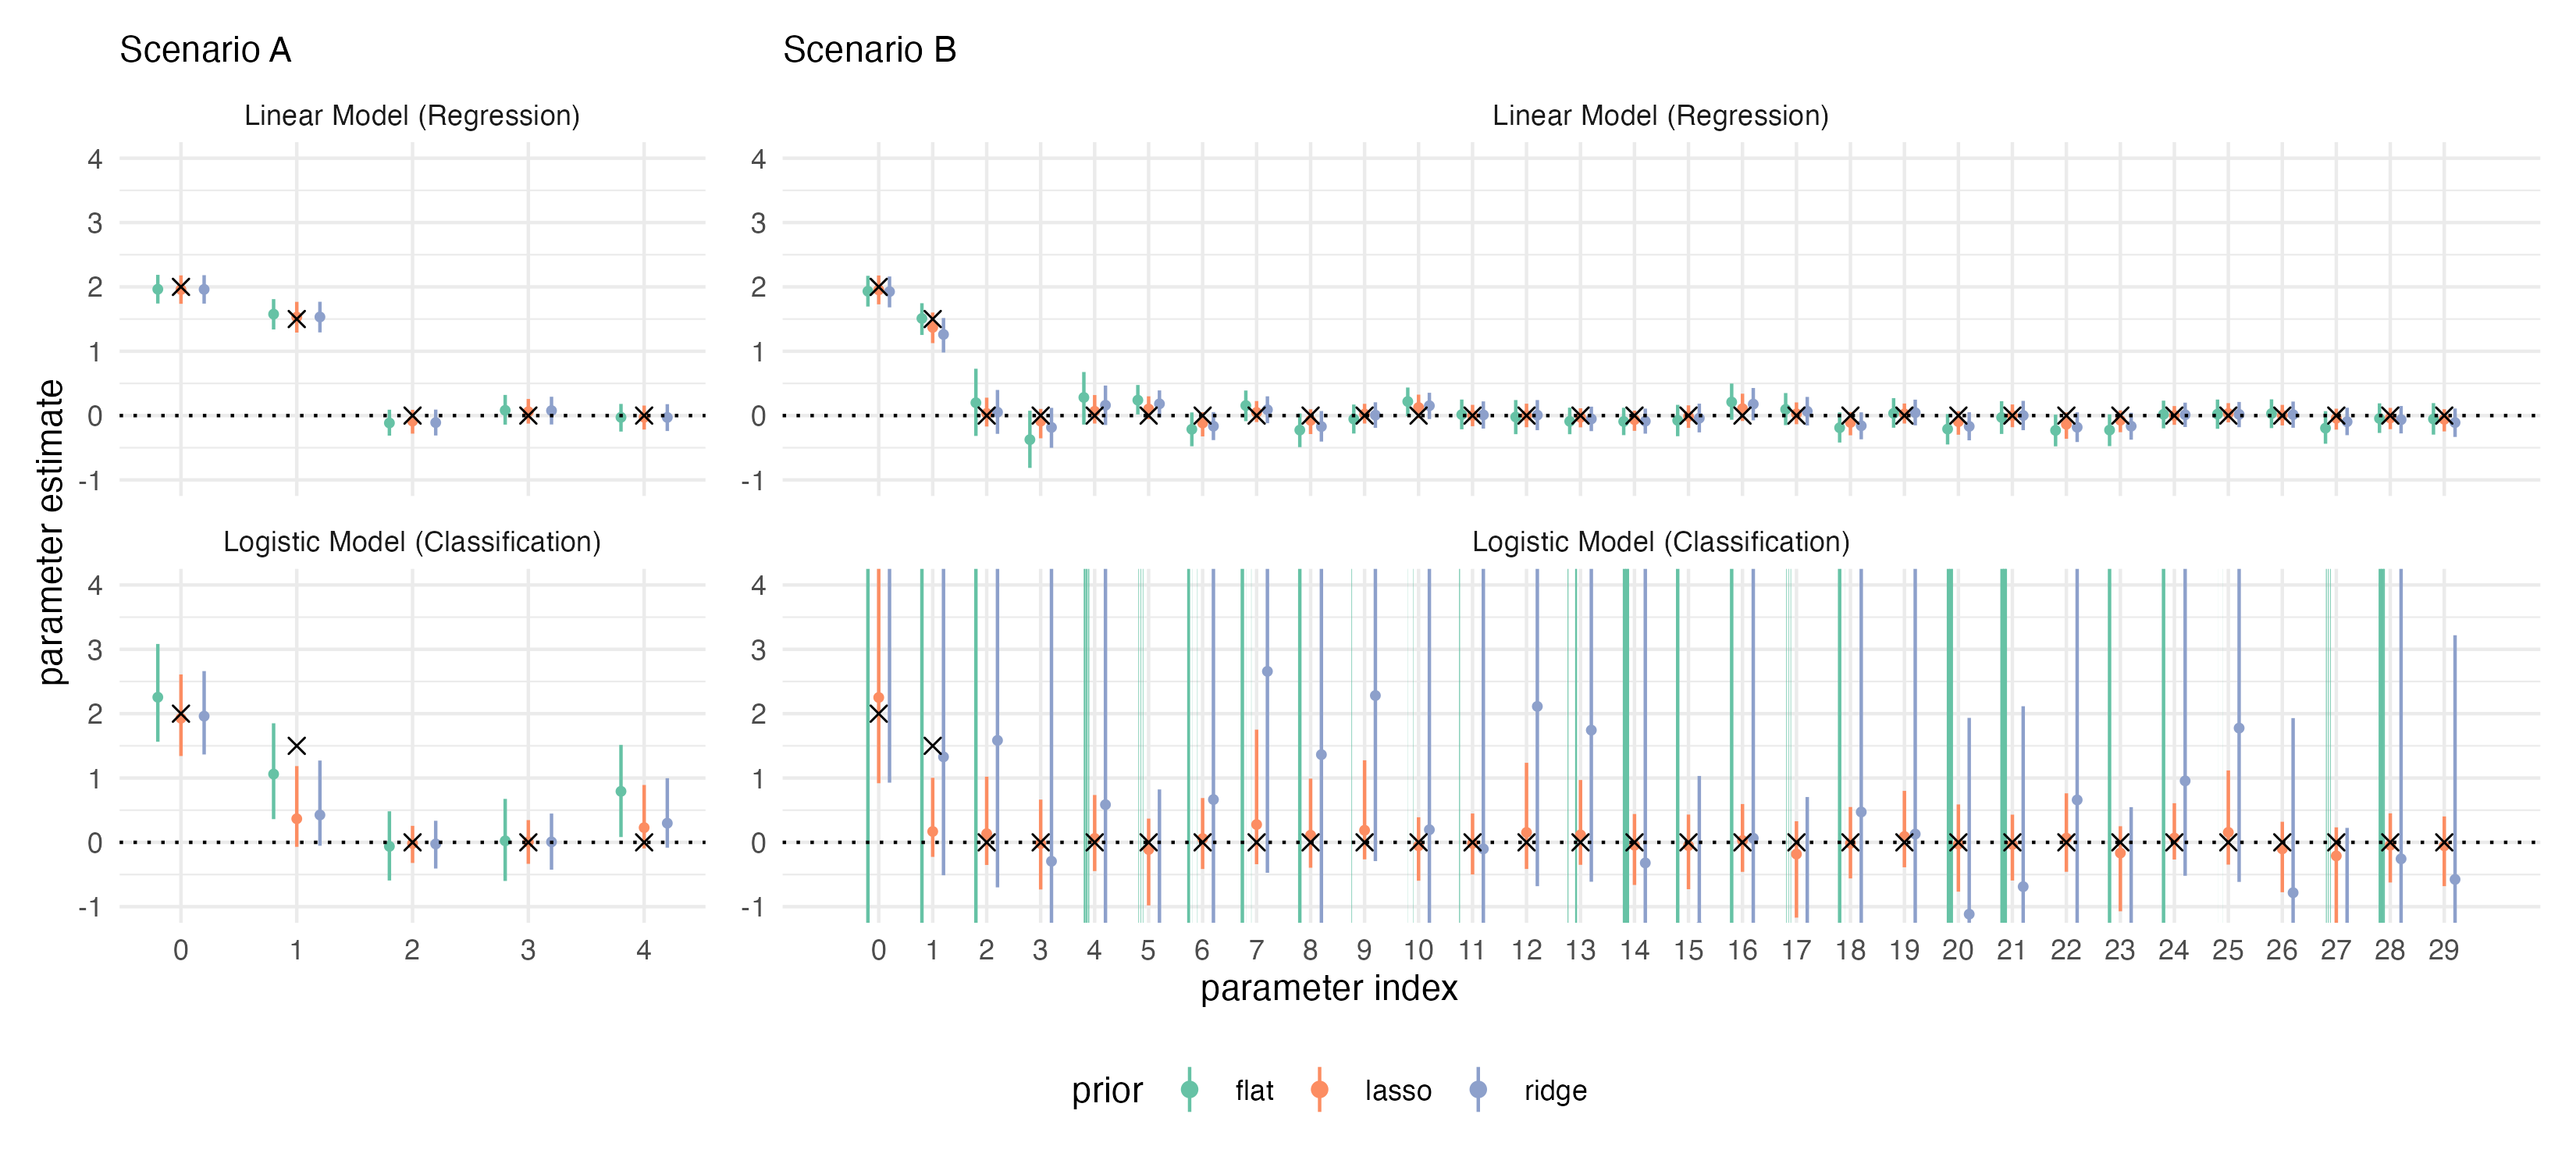
\includegraphics[width=\linewidth]{../figures/reg_all.png}
    \caption{Estimated model parameters with 95\% credibility intervals (CI). True parameter values are shown as black crosses. Linear models yielded more accurate estimates with narrower CIs than logistic models. In Scenario B, the uncertainty of the unregularized logistic model becomes especially pronounced, illustrating the need for regularization in high-dimensional, low-information settings.
    }
    \label{fig:reg-params}
\end{figure}

\subsection{Performance of approximate inference algorithms in Bayesian regression}

In this second experiment, we compared Laplace Approximation (LA) and Metropolis-Hastings MCMC in Bayesian linear and logistic regression.\\

We generate 1,000 synthetic data sets with $n=100$:
\begin{equation*}
    \begin{aligned}
        &\bX \sim \Ncal(\bnull, \bI), \quad \btheta = (-0.5, 2, 1)\\
        &\text{linear: } \by \mid \btheta \sim \Ncal(\bX \btheta, \bI),\quad \text{logistic: } \by \mid \btheta \sim \text{Ber}(\sigma(\bX \btheta))
    \end{aligned}
\end{equation*}

Each dataset was used to fit one linear and one logistic model, using both inference approaches.
We assumed $\btheta \sim \Ncal(0, 10 \bI)$ and fixed residual variance $\ssd = 10$.
For LA, we used \texttt{r-INLA} with settings to default from INLA to simple LA.
For MCMC, we used the \texttt{MCMCglmm} package with settings specifically to use Metropolis Hastings, a relatively small sample size of 5,000, a burnin periord of 500 and a thinning interval of 10.
For each method, we recorded CPU runtime, posterior means, and posterior standard deviations of the estimated parameters.\\

\begin{figure}[htbp]
    \centering
    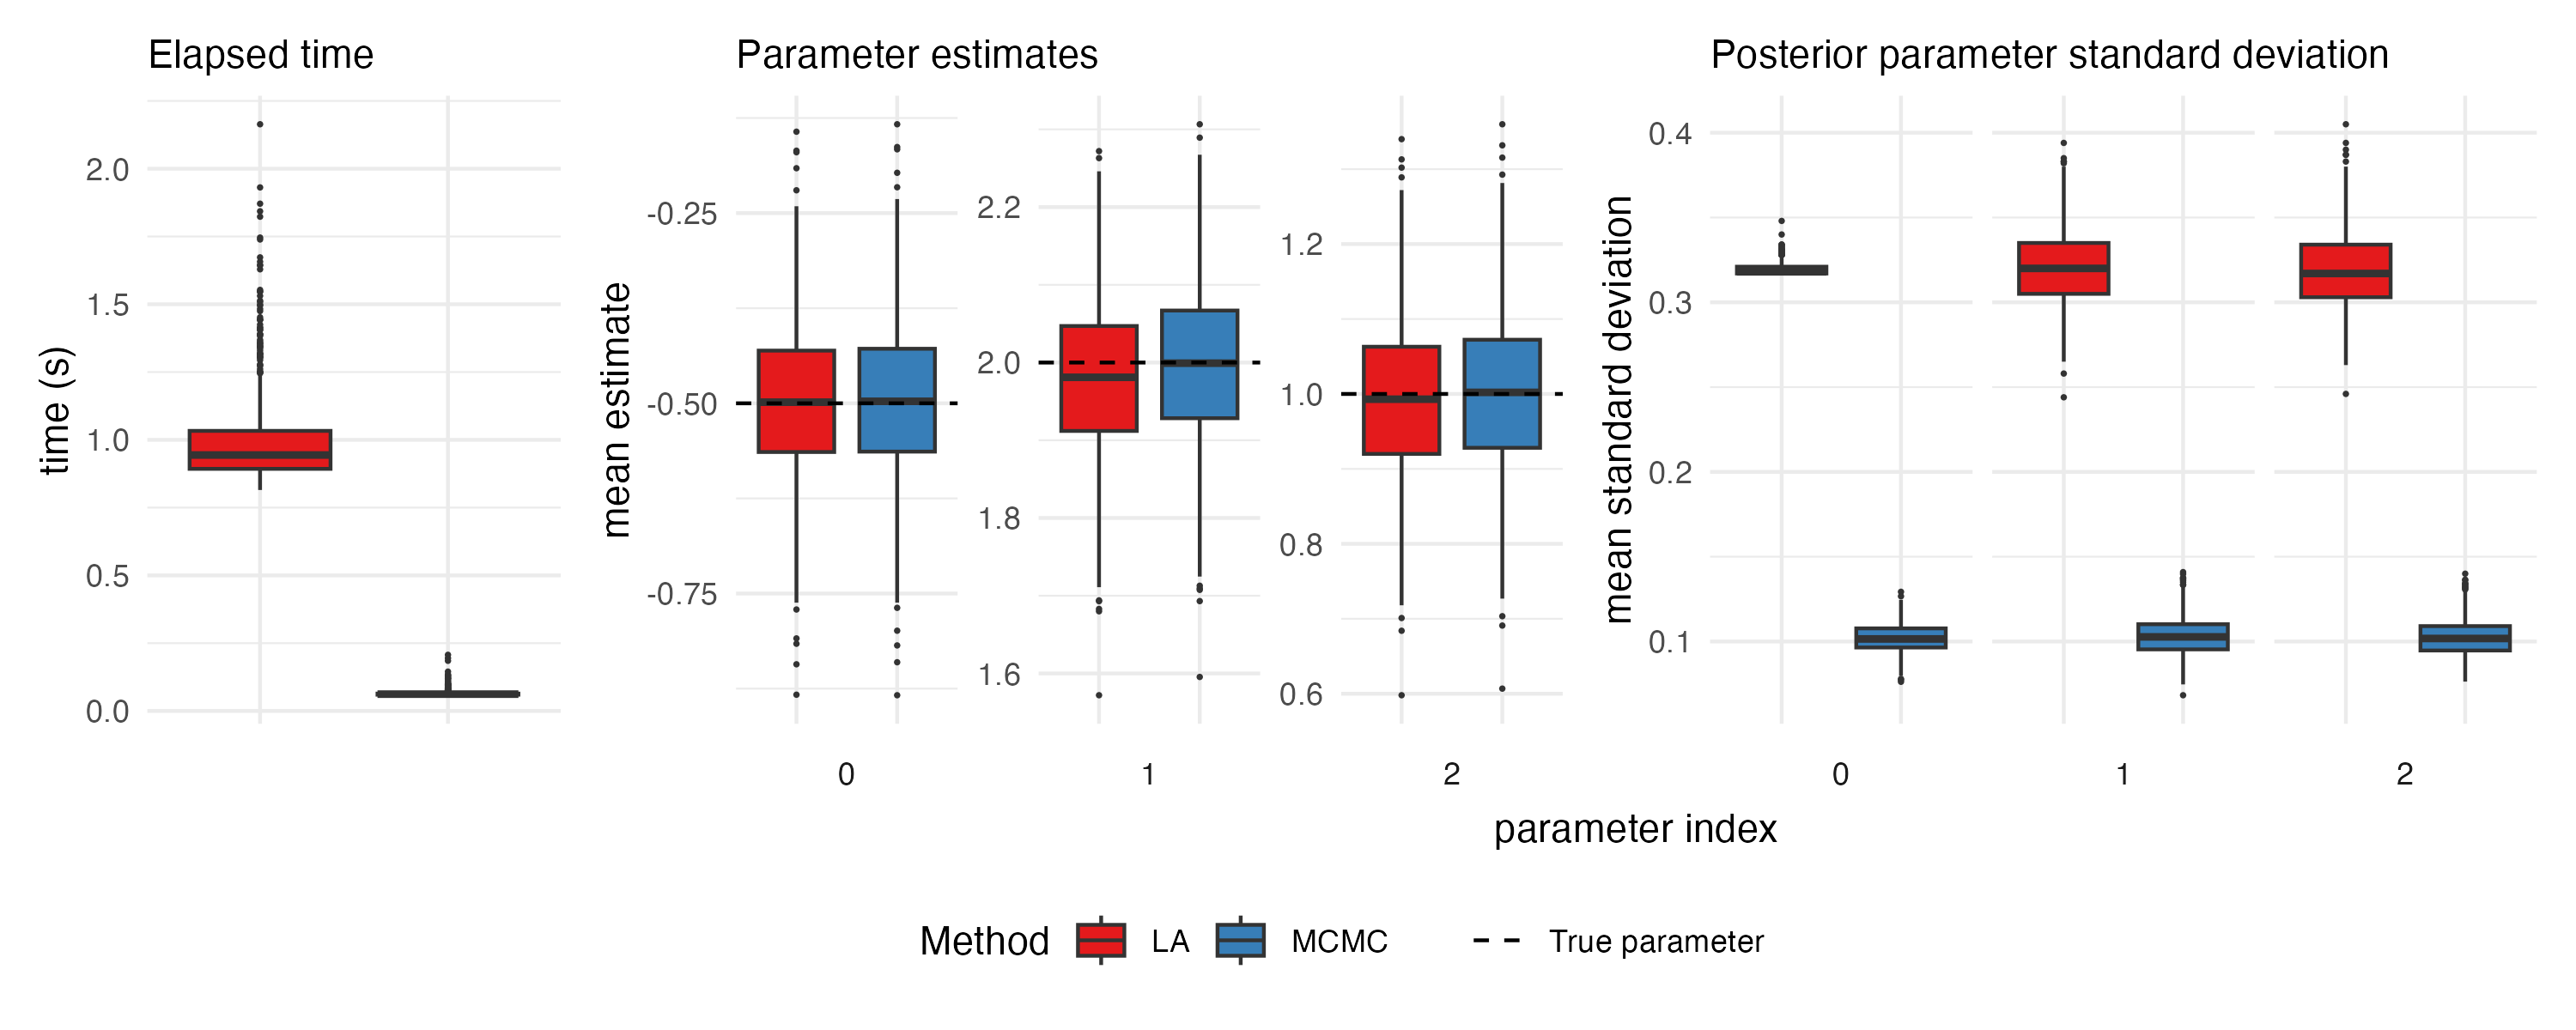
\includegraphics[width=\linewidth]{../figures/approx_regr.png}
    \caption{
    Bayesian linear regression: Comparison of LA (red) and MCMC (blue) across 1,000 simulations. MCMC is faster in this setting. Both methods estimate parameters accurately, though LA yields higher posterior uncertainty. 
    }
    \label{fig:approx-regr}
\end{figure}

\begin{figure}[htbp]
    \centering
    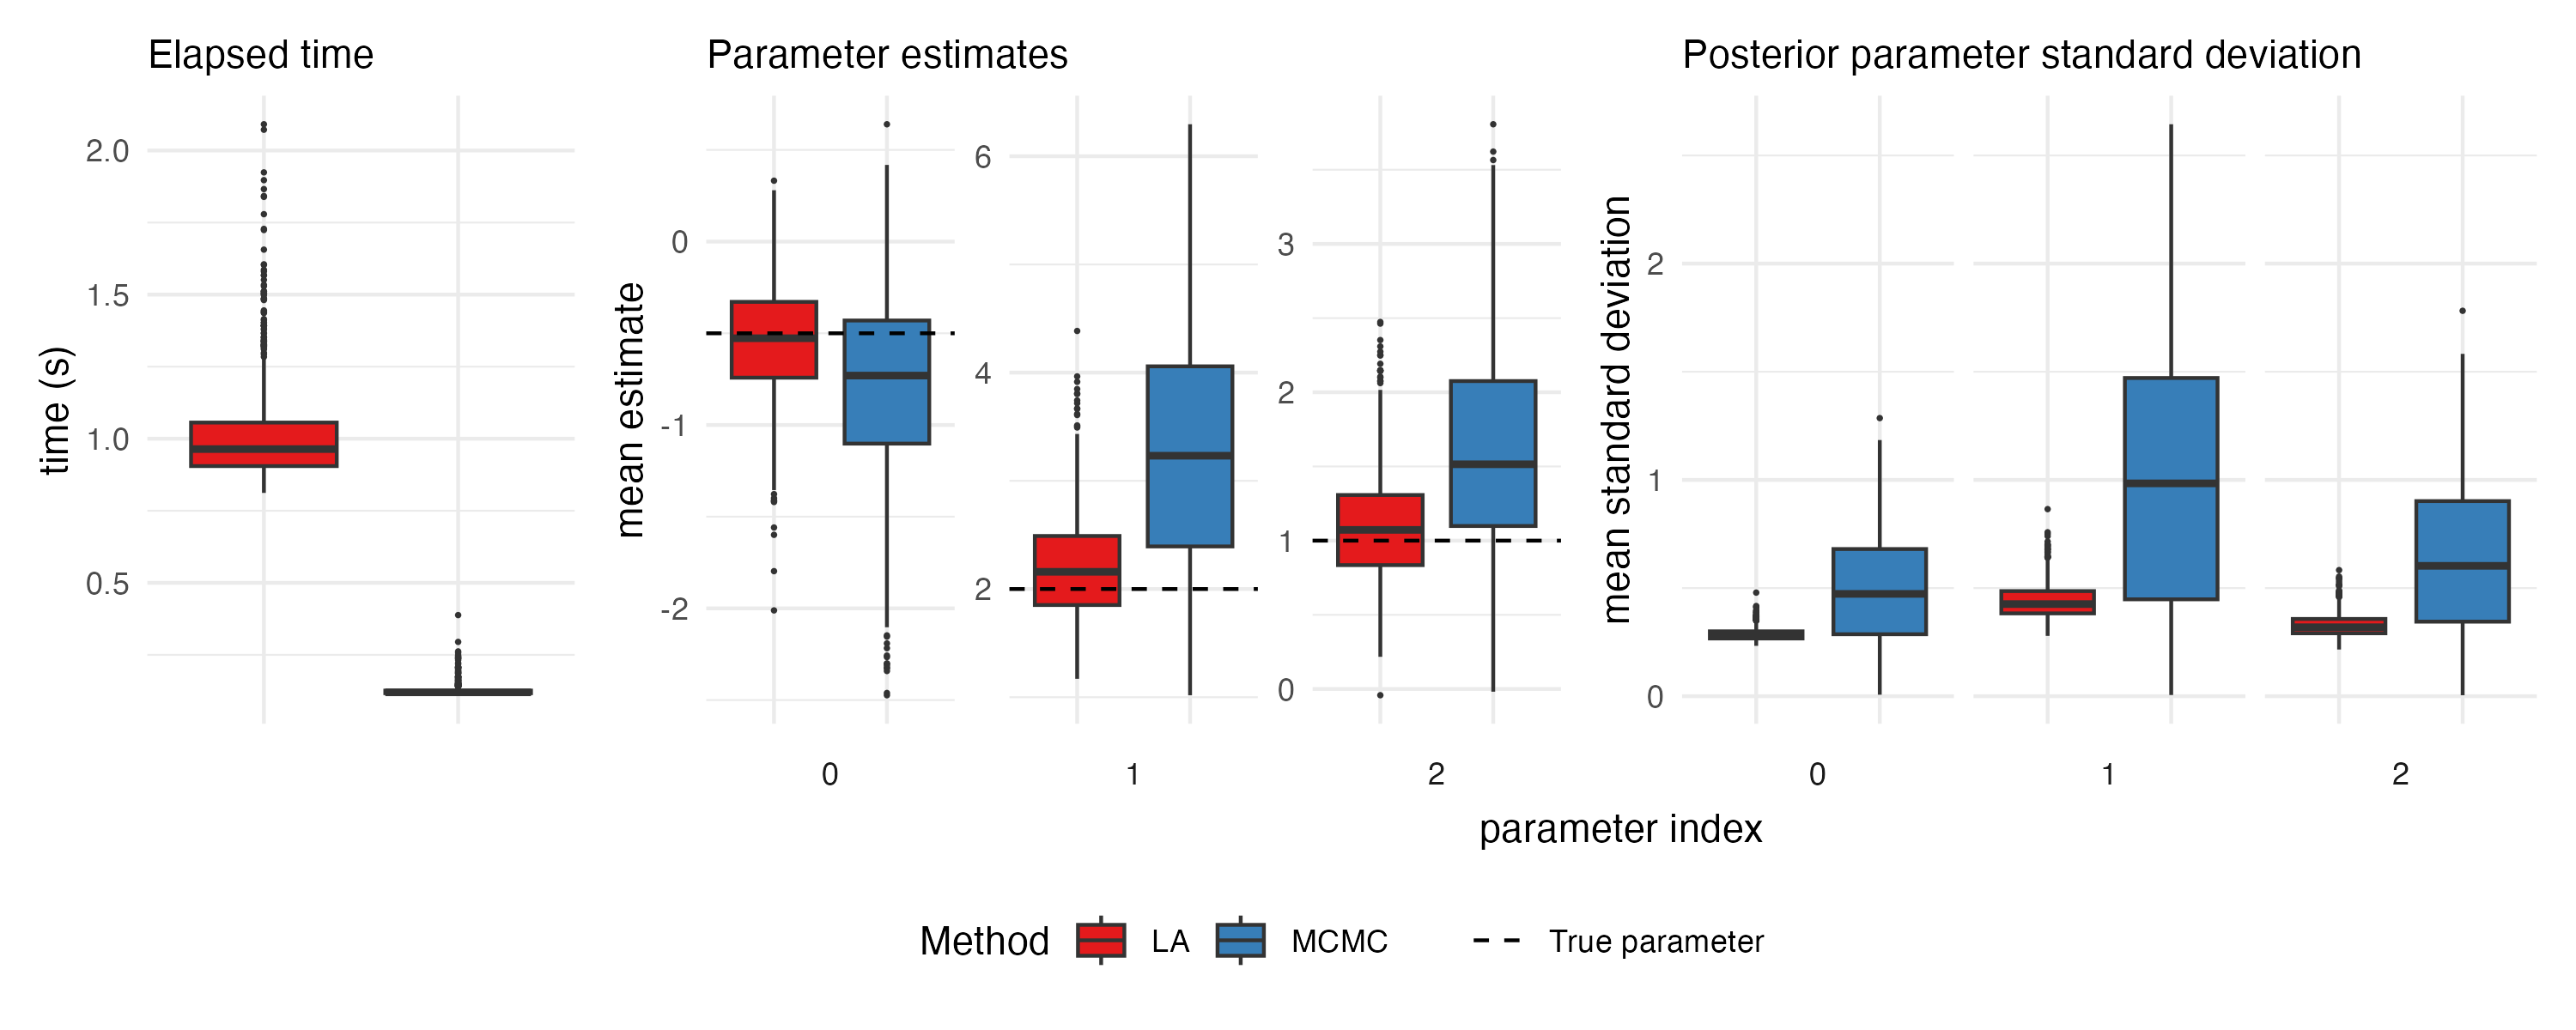
\includegraphics[width=\linewidth]{../figures/approx_class.png}
    \caption{
    Bayesian logistic regression: Comparison of LA (red) and MCMC (blue) across 1,000 simulations. LA outperforms MCMC in both accuracy and precision of parameter estimates. While LA is slower to compute, it provides more stable estimates.
    }
    \label{fig:approx-class}
\end{figure}

Results for the linear and logistic model can be seen in \autoref{fig:approx-regr} and \autoref{fig:approx-class} respectively.
In our experiment, LA was generally slower than MCMC methods.
In the case of the Bayesian linear model (\autoref{fig:approx-regr}), there was not much difference in the posterior parameter estimates, although LA leads to much higher standard deviation of parameters.
In contrast, LA showed clear advantages in logistic regression (\autoref{fig:approx-class}): it yielded more accurate parameter estimates and lower posterior uncertainty than MCMC. These results highlight that the performance of approximate inference methods can differ significantly depending on the model and likelihood.



\newpage

\section{Conclusion and Outlook}
\label{sec:conclusion}
A concise summary of contents and results

\newpage

% ------------------------------------------------------------------------------
% APPENDIX ---------------------------------------------------------------------
% ------------------------------------------------------------------------------

\pagenumbering{Roman}

\setcounter{page}{5} % CHANGE

\appendix

\section{Appendix}
\label{sec:app}
\subsection*{Notation}

We denote prior parameters with $\breve{}$ and posterior parameters with $\post{}$. Vectors are written in bold-face like so $\bx$ and matrices are bold capital letters $\bX$.

\begin{itemize}
    \item[$\btheta$] regression weights
    \item[] 
\end{itemize}



\subsection*{Distributions}

When deriving equations, we assume the following probability density functions and parameter placements:

\begin{itemize}
    \item[$\Ncal(\mu, \ssd)$] Gaussian distribution with mean $\mu$ and variance $\ssd$
    \item[] Gamma distribution
    \item[$IG(a, b)$] Inverse Gamma distribution with scale parameter $a$ and location parameter $b$
    \item[]  (multivariate) Student t-distribution
    \item[] 
\end{itemize}

\subsection*{Proofs and Derivations}

\subsubsection*{Posterior of the Normal-Inverse-Gamma prior}
For the model described in \eqref{eq:NIGprior}, the posterior distribution is calculated according to \citet{fahrmeir_regression_2021} as
\begin{equation*}
    \begin{aligned}
        p(\btheta, \ssd \mid \by) &\overset{\eqref{eq:bayes}}{\propto} \Lcal(\btheta, \ssd \mid \by) p(\btheta, \ssd) \\
        &= \Lcal(\btheta, \ssd \mid \by) p(\btheta \mid \ssd) p(\ssd) \\
        &= \frac{1}{(\ssd)^{n/2}} \exp\bigl( - \frac{1}{2\ssd} (\by - \bX \btheta)^\top(\by - \bX \btheta) \bigr)\\
        &= \frac{1}{(\ssd)^{p/2}} \exp\bigl( - \frac{1}{2\ssd} (\btheta - \mupri)^\top \Sdipri (\btheta - \mupri) \bigr)\\
        &= \frac{1}{(\ssd)^{\apri + 1}} \exp\bigl( - \frac{\bpri}{\ssd} \bigr),
    \end{aligned}
\end{equation*}

which is NIG-distributed

\begin{equation*}
    \btheta, \ssd \mid \by \sim \text{NIG}(\mupo, \Sdpo, \apo, \bpo)
\end{equation*}

with parameters

\begin{equation*}
    \begin{aligned}
        \mupo &= \Sdpo (\Sdipri \mupri + \bX^\top \by) \\
        \Sdpo &= (\bX^\top \bX + \Sdipri)^{-1} \\
        \apo &= \apri + \frac{n}{2}\\
        \bpo &= \bpri + \frac{1}{2} ( \by^\top \by + \mupri^\top \Sdipri \mupo - \mupo^\top \Sdipo \mupo).
    \end{aligned}
\end{equation*}

For the conditional posteriors it holds that
\begin{equation*}
    \begin{aligned}
        \btheta \mid \ssd, \by &\sim \Ncal(\mupo, \ssd \Sdpo) \\
        \btheta \mid \by &\sim \Tcal(2 \apo, \mupo, \bpo / \apo \Sdpo).
    \end{aligned}
\end{equation*}

\newpage

\section{Electronic Appendix}
\label{sec:el_app}

Data, code, and figures are provided in electronic format. All figures and scripts can be accessed at \url{https://github.com/lona-k/bayesian-GLMs-seminar}.

\newpage

% ------------------------------------------------------------------------------
% BIBLIOGRAPHY -----------------------------------------------------------------
% ------------------------------------------------------------------------------

\RaggedRight
\bibliographystyle{dcu}
\bibliography{bibliography}

\subsection*{Research Instruments}

All thoughts presented in this paper are my own, unless otherwise noted.
Neither ChatGPT \citep{chatgpt} nor any other LLM directly wrote the text for any part of this paper.
Throughout this work, I used Grammarly \citep{grammarly} to improve and proof-read the text.

ChatGPT  was used, alongside traditional research methods, as a starting point for finding further relevant literature (such as the original author and paper establishing a method, \citet[e.g.][]{tibshirani_regression_1996} for the LASSO method).
Despite this, all listed sources have been read and checked by me before using and referencing them in this work.
ChatGPT was also used as a conversation partner for helping me understand difficult parts of papers and theories and coming to terms with the philosophical ideas behind Bayesian statistics.
ChatGPT was consulted, although sparingly and with little helpful results, about some errors in the code for the examples in this paper.
More abstractly, I used ChatGPT to format this document and to help me solve difficult \LaTeX errors, such as issues with automated citations and rendering.

\newpage

% ------------------------------------------------------------------------------
% DECLARATION OF AUTHORSHIP-----------------------------------------------------
% ------------------------------------------------------------------------------

\Large
\noindent
\textbf{Declaration of Authorship}
\vspace{0.5cm}
\noindent
\normalsize

I hereby declare that the report submitted is my own unaided work. All direct
or indirect sources used are acknowledged as references. I am aware that the
Thesis in digital form can be examined for the use of unauthorized aid, and in
order to determine whether the report as a whole or parts incorporated in it may
be deemed as plagiarism. For the comparison of my work with existing sources, I
agree that it shall be entered in a database where it shall also remain after
examination, to enable comparison with future Theses submitted. Further rights
of reproduction and usage, however, are not granted here. This paper was not
previously presented to another examination board and has not been published.
\\

\vspace{1cm}
\textcolor{orange}{Location, date} \\

\vspace{3cm}

\noindent\rule{0.5\textwidth}{0.4pt} \\

\textcolor{orange}{Name}

% ------------------------------------------------------------------------------

\end{document}
